In this chapter we discuss our approach to analyzing high-throughput genomic
datasets through deep analysis pipelines, and its implementation in 
walrus.\cite{walrus} We also evaluate the performance of walrus and show its
usefulness in a precision medicine setting. While walrus was developed in this
context we also show its usefulness in other areas, specifically for
\gls{rna}-seq analyses. 

\section{Use Case and Motivation} 
For cancer, high throughput sequencing is the main technology to facilitate
personalized diagnosis and treatment since it enables collecting high quality
genomic data from patients at a low cost. 
Analyzing sequencing datasets require deep analysis pipelines with a large
number of steps that transform raw data into interpretable
results.\cite{diao2015building} These pipelines often consists of in-house or
third party tools and scripts that each transform input files and produce some
output. Although different tools exist, it is necessary to carefully explore
different tools and parameters to choose the most efficient to apply for a
dedicated question.\cite{servant2014bioinformatics} The complexity of the tools
vary from toolkits such as the \gls{gatk} to small custom \emph{bash} or
\emph{R} scripts.  In addition some tools interface with databases whose
versions and content will impact the overall result.\cite{sboner2015primer}

When developing analysis pipelines for use in precision medicine it is necessary
to track pipeline tool versions, their input parameters, and data. Both to
thoroughly document what produced the end results, but also to compare results
from different pipeline runs.  Because of the iterative process of developing
the analysis pipeline, thoroughly investigating emerging patterns and
signatures, it is necessary to use analysis tools that facilitates modifying
pipeline steps and adding new ones with little developer effort. 

We have previously analyzed DNA sequence data from a breast cancer patient's
primary tumor and adjacent normal cells to identify the molecular signature of
the patient's tumor and germline. When the patient later relapsed we analyzed
sequence data from the patient's metastasis to provide an extensive comparison
against the primary and to identify the molecular drivers of the patient's
tumor. 

For the initial \gls{wgs} analysis we developed a pipeline to investigate
somatic and germline mutations based on Broad Institute's best practices. We
developed the analysis pipeline on our in-house compute server using a
\emph{bash} script version controlled with \emph{git} to track changes as we
developed the analysis pipeline. The pipeline consisted of tools including
picard,\footnote{\url{broadinstitute.github.io/picard}}
fastqc,\footnote{\url{bioinformatics.babraham.ac.uk/projects/fastqc}}
trimmomatic,\footnote{\url{usadellab.org/cms/?page=trimmomatic}} and the
\gls{gatk}.\footnote{\url{software.broadinstitute.com/gatk}} While the analysis
tools themselves provide the necessary functionality to give insights in
the disease, ensuring that the analyses could be fully reproduced later left
areas in need of improvement.

We chose a command-line script over more complex pipelining tools or workbenches
such as Galaxy\cite{galaxy} because of its fast setup time on our available
compute infrastructure, and familiar runtime. More complex systems could be
beneficial in larger research groups with more resources to compute
infrastructure maintenance, whereas command-line scripting languages require
little to none over normal use. In addition, while there are off-site solutions
for executing scientific workflows, analyzing sensitive data often put hard
restrictions on where the data can be stored an
analyzed.

After we completed the first round of analyses we summarized our efforts and
noted some lessons learned. 
First, datasets and databases should be version
controlled and stored along with the pipeline description. In the analysis
script we referenced to datasets and databases by their physical location on a
storage system, but these were later moved without updating the pipeline
description causing extra work. A solution would be to add the data to the same
version control repository hosting the pipeline description.
Second, the specific pipeline tools should also be kept available for later use.
Since installing many bioinformatics tools require a long list of dependencies,
it is beneficial to store the pipeline tools to reduce the time to start
analyzing new data or re-run analyses. 
Another lesson is that it should be easy to add new tools to an existing
pipeline and execution environment. This includes installing the specific tool
and adding to an existing pipeline.  Bundling tools within software containers,
such as Docker, and hosting them on an online registry simplifies the tool
installation process since the only requirement is the container runtime.
Another lesson learned is that while bash scripts have
their limitations, using a well-known format that closely resembles the normal
command-line use clearly have its advantages. It is easy to understand what
tools were used, their input parameters, and the data flow. However, from our
experience when these analysis scripts grow too large they become too complex to
modify and maintain. 

The above problem areas are not just applicable to our research group, but
common to other projects as well. Especially when hospitals and research groups
aim to apply personalized medicine efforts to guide therapeutic strategies and
diagnosis, the analyses will have to be able to be easily reproducible later. We
used the lessons learned to  design and implement \emph{walrus}, a command line
tool for developing and running data analysis pipelines. It automatically
orchestrates the execution of different tools, and tracks tool versions and
parameters, as well as datasets through the analysis pipelines pipeline. It
provides users a simple interface to inspect differences in pipeline runs, and
retrieve previous analysis results and configurations. In the remainder of the
paper we describe the design and implementation of walrus, its clinical use, its
performance, and how it relates to other pipeline managers. 


\section{\texttt{walrus}} 
walrus is a tool for developing and executing data analysis pipelines. It stores
information about tool versions, tool parameters, input data, intermediate data,
output data, as well as execution environments to simplify the process of
reproducing data analyses. Users write descriptions of their analysis pipelines
using a familiar syntax and walrus uses this description to orchestrate the
execution of the pipeline. In walrus we package all tools in software
containers to capture the details of the different execution environments. While
we have used walrus to analyse high-throughput datasets in precision medicine,
it is a general tool that can analyze any type of data, e.g. image datasets for
machine learning. It has few dependencies and runs on on any platform that
supports Docker containers, it can even run in a container itself.  While other
popular pipeline managers require the use of cluster computers or cloud
environment, we focus on single compute nodes often found in clinical
environments such as hospitals. 

walrus is implemented as a command-line tool in the Go programming language. We
use the popular software container implementation
Docker\footnote{\url{docker.com}} to provide reproducible execution
environments, and interface with git together with
git-lfs\footnote{\url{git-lfs.github.com}} to version control datasets and
pipeline descriptions. By choosing Docker and git we have built a tool that
easily integrates with current bioinformatic tools and workflows. 

With walrus we target pipeline developers that use command-line tools and
scripting languages to build and run analysis pipelines. Users wrap their
existing tools in Docker containers and can use their existing compute
infrastructure.  We integrate with the current workflow using git to version
control analysis scripts, and use git-lfs to expand to versioning of datasets as
well. We have designed the pipeline description format resembles the command
line syntax as much as possible. 



\subsection{Pipeline Configuration}
Users configure analysis pipelines by writing pipeline description files in a
human readable format such as \gls{json} or \gls{yaml}. A pipeline description
contains a list of stages, each with inputs and outputs, along with optional
information such as comments or configuration parameters such as caching rules
for intermediate results. Listing \ref{examplelisting} shows an example pipeline
stage that uses MuTect\cite{mutect} to detect somatic point mutations. Users
can also specify the tool versions 

Users specify the flow of data in the pipeline within the pipeline description,
as well as the dependencies between the steps. Since pipeline configurations can
become complex, walrus provides a plotting tool for visualizing the pipeline
using tools such as Graphviz.\footnote{\url{graphviz.org}} before running the
pipeline. 


\begin{lstlisting}[caption={Example pipeline stage for a tool that detects
somatic point mutations. It reads a reference sequence file together with both
tumor and normal sequences, and produces an output file with the detected
mutations.},
label={examplelisting}, 
basicstyle=\ttfamily\scriptsize]
        {
          "Name": "mutect",
          "Image": "fjukstad/mutect:1.1.7",
          "Cmd": [
            "--analysis_type","MuTect",
            "--reference_sequence","/walrus/input/reference.fasta",
            "--input_file:normal","/walrus/input/normal.bam",
            "--input_file:tumor","/walrus/input/tumor.bam",
            "-L","/walrus/input/targets.bed",
            "--out","/walrus/mutect/mutect-stats-txt",
            "--vcf","/walrus/mutect/mutect.vcf"
          ],
          "Inputs":[
             "input" 
          ]
        }
\end{lstlisting}

Users add data to an analysis pipeline by simply specifying the location of the
input data in the pipeline description, and walrus automatically mounts it to
the container running the analysis. The location of the input files can either
be local or remote locations such as an FTP server. When the pipeline is
completed, walrus will store all the input, intermediate and output data to a
user-specified location.  

\subsection{Pipeline Execution}
When users have written a pipeline description for their analyses, they can use
the command-line interface of walrus to run the analysis pipeline. 
walrus builds an execution plan from the pipeline description and runs it for
the user. It uses the input and output fields of each pipeline stage to
construct a \gls{dag} where each node is a pipeline stage and the links are
input/output data to the stages. From this graph walrus can determine
parallelizable stages and coordinate the execution of the pipeline.

In walrus, each pipeline stage is run in a separate container, 
and users can specify container versions in the pipeline description to specify
the correct version of a tool. We treat a
container as a single executable and users specify tool input arguments in the
pipeline description file using standard command line syntax. walrus will
automatically build or download the container images with the analysis tools,
and start these with the user-defined input parameters and mount the appropriate
input datasets. While the pipeline is running, walrus monitors running stages
and schedules the execution of subsequent pipeline stages when their respective
input data become available. We have designed walrus to execute an analysis
pipeline on a single large server, but since the tools are run within
containers, these can easily be orchestrated across a range of servers in future
versions. 

Users can select from containers with bioinformatics tools installed or build
their own using a standard Dockerfile. Through software containers walrus can
provide a reproducible execution environment for the pipeline, and containers
provide simple execution on a wide range of software and hardware platforms.
With initiatives such as BioContainers,\cite{biocontainers} researchers can make
use of already existing containers without having to re-write their own. Data in
each pipeline step is automatically mounted and made available within each
Docker container. By simply relying on Docker walrus requires little software
setup to run different bioinformatics tools. 

While walrus executes a single pipeline on one physical server, it supports both
data and tool parallelism, as well as any parallelization strategies within each
tool, e.g. multi-threading. If users want to run the same analyses for a set of
samples, or for example per chromosome, they can simply list the samples in the
pipeline description and walrus will automatically run each sample through the
pipeline in parallel. While we can parallelize the independent pipeline steps,
the performance of an analysis pipeline relies on the underlying tools and
available compute power. This also applies to the scalability of the analysis
pipeline. 

Upon successful completion of a pipeline run, walrus will write a verbose
pipeline description file to the output directory. This file contains
information on the runtime of each step, which steps were parallelized, and
provenance related information to the output data from each step. Users can
investigate this file to get a more detailed look on the completed pipeline. In
addition to this output file walrus will return a version ID for the pipeline
run, which later can be used to investigate a previous pipeline run. 

\subsection{Data Management}
In walrus we provide an interface for users to track their analysis data with a
version control system. This allows users to inspect data from previous pipeline
runs without having to recompute all the data. walrus stores all intermediate
and output data in an output directory specified by the user, which is version
controlled automatically by walrus when new data is produced by the pipeline. 

In walrus we interface with git to track any output file from the analysis
pipeline. When users start running a pipeline walrus will look for a git
repository in the same directory as the pipeline description, if it cannot find
a repository it will create one for the user. As pipeline stages complete,
walrus will automatically add and commit the output files for each stage to the
git repository, using git-lfs to track datasets. Users typically use a single
repository per pipeline, but can use the same repository to version multiple
pipelines as well. With git-lfs, instead of writing large blobs to a repository
it writes small pointer files that contains the hash of the original file, the
size of the file, and the version of git-lfs used. The files themselves are
stored separately which makes the size of the repository small and manageable
with git. The main reason why we chose git and git-lfs for version control is
that git is the de facto standard for versioning source code, and we want to
include versioning of datasets without altering the typical development
workflow. 

Since we are working with potentially sensitive datasets walrus is targeted at
users that use a local compute and storage servers. It is up to users to
configure a remote tracker for their repositories, but we provide command-line
functionality in walrus to run a git-lfs server that can store users' contents.
They can use their default remotes, such as Github, for hosting source code but
they must themselves provide the remote server to host their data.

\subsection{Pipeline Reconfiguration and Re-execution}
Reconfiguring a pipeline is common practice in precision medicine, e.g. if we
later would like to change tool parameters or add additional steps to the
analysis pipeline. To reconfigure an existing pipeline users make the applicable
changes to the pipeline description and re-run it using walrus. walrus will then
recompute the necessary steps and return a version ID for the newly run
pipeline. This ID can be used to compare pipeline runs, the changes made, and
optionally restore the data and configuration from a previous run. 
Reconfiguring the pipeline to use updated tools or reference genomes will alter
the pipeline configuration and force walrus to recompute the applicable pipeline
stages. 

The command-line interface of walrus provides functionality to restore results
from a previous run, as well as printing information about a completed pipeline.
To restore a previous pipeline run, users use the \texttt{restore} command in
walrus together with the version ID of the respective pipeline run. walrus will
interface with git to restore the files to their state at the necessary point in
time.

\section{Evaluation}
To evaluate the usefulness of walrus we demonstrate its use in a clinical
setting, and the low computational time and storage overhead to support
reproducible analyses.

\subsection{Clinical Application} 
We have used walrus to analyze a whole-exome dataset to from a sample in the
McGill Genome Quebec [MGGQ] dataset (GSE58644)\cite{tofigh2014prognostic} to
discover \glspl{snp}, genomic variants and somatic mutations. We interactively
developed a pipeline description that follows the best-practices of The Broad
Institute\footnote{\url{software.broadinstitute.org/gatk/best-practices}} and
generated reports that summarized the findings to share the results. 

From the analyses we discovered inherited germline mutations that are recognized
to be among the top 50 mutations associated with an increased risk of familial
breast cancer. We also discovered a germline deletion which has been associated
with an increased risk of breast cancer. We also discovered mutations in a
specific gene that might explain why specific drug had not been effective in the
treatment of the primary tumor. From the profile of the primary tumor we
discovered many somatic events (around 30 000) across the whole genome with
about 1000 in coding regions, and 500 of these were coding for non-synonymous
mutations.  We did not see amplification or constituent activation of growth
factors like HER2, EGFR or other players in breast cancer. Because of the
germline mutation, early recurrence, and lack of DNA events, we suspect that the
patient's primary tumor was highly immunogenic. We have also identified several
mutations and copy number changes in key driver genes. This includes a mutation
in a gene that creates a premature stop codon, truncating one copy of the gene.

While we cannot share the results in details or the sensitive dataset, we have
made the pipeline description available at \url{github.com/uit-bdps/walrus}
along with other example pipelines. 

\subsection{Performance and Resource Usage}
To demonstrate the performance of walrus and the ability to track and detect
changes in an analysis pipeline, we have implemented one of the variant calling
pipelines from \cite{cornish2015comparison} using tools from picard
and the \gls{gatk}. We show the storage and computational overhead of our
approach, and the benefit of capturing the pipeline specification using a
pipeline manager rather than a methods section in a paper. 
The pipeline description, data, and code is available along with walrus at
\url{github.com/uit-bdps/walrus}. We use the popular NA12878 dataset since it
makes it possible to easily share both the pipeline description and resulting
datasets. 

% \begin{figure}
% 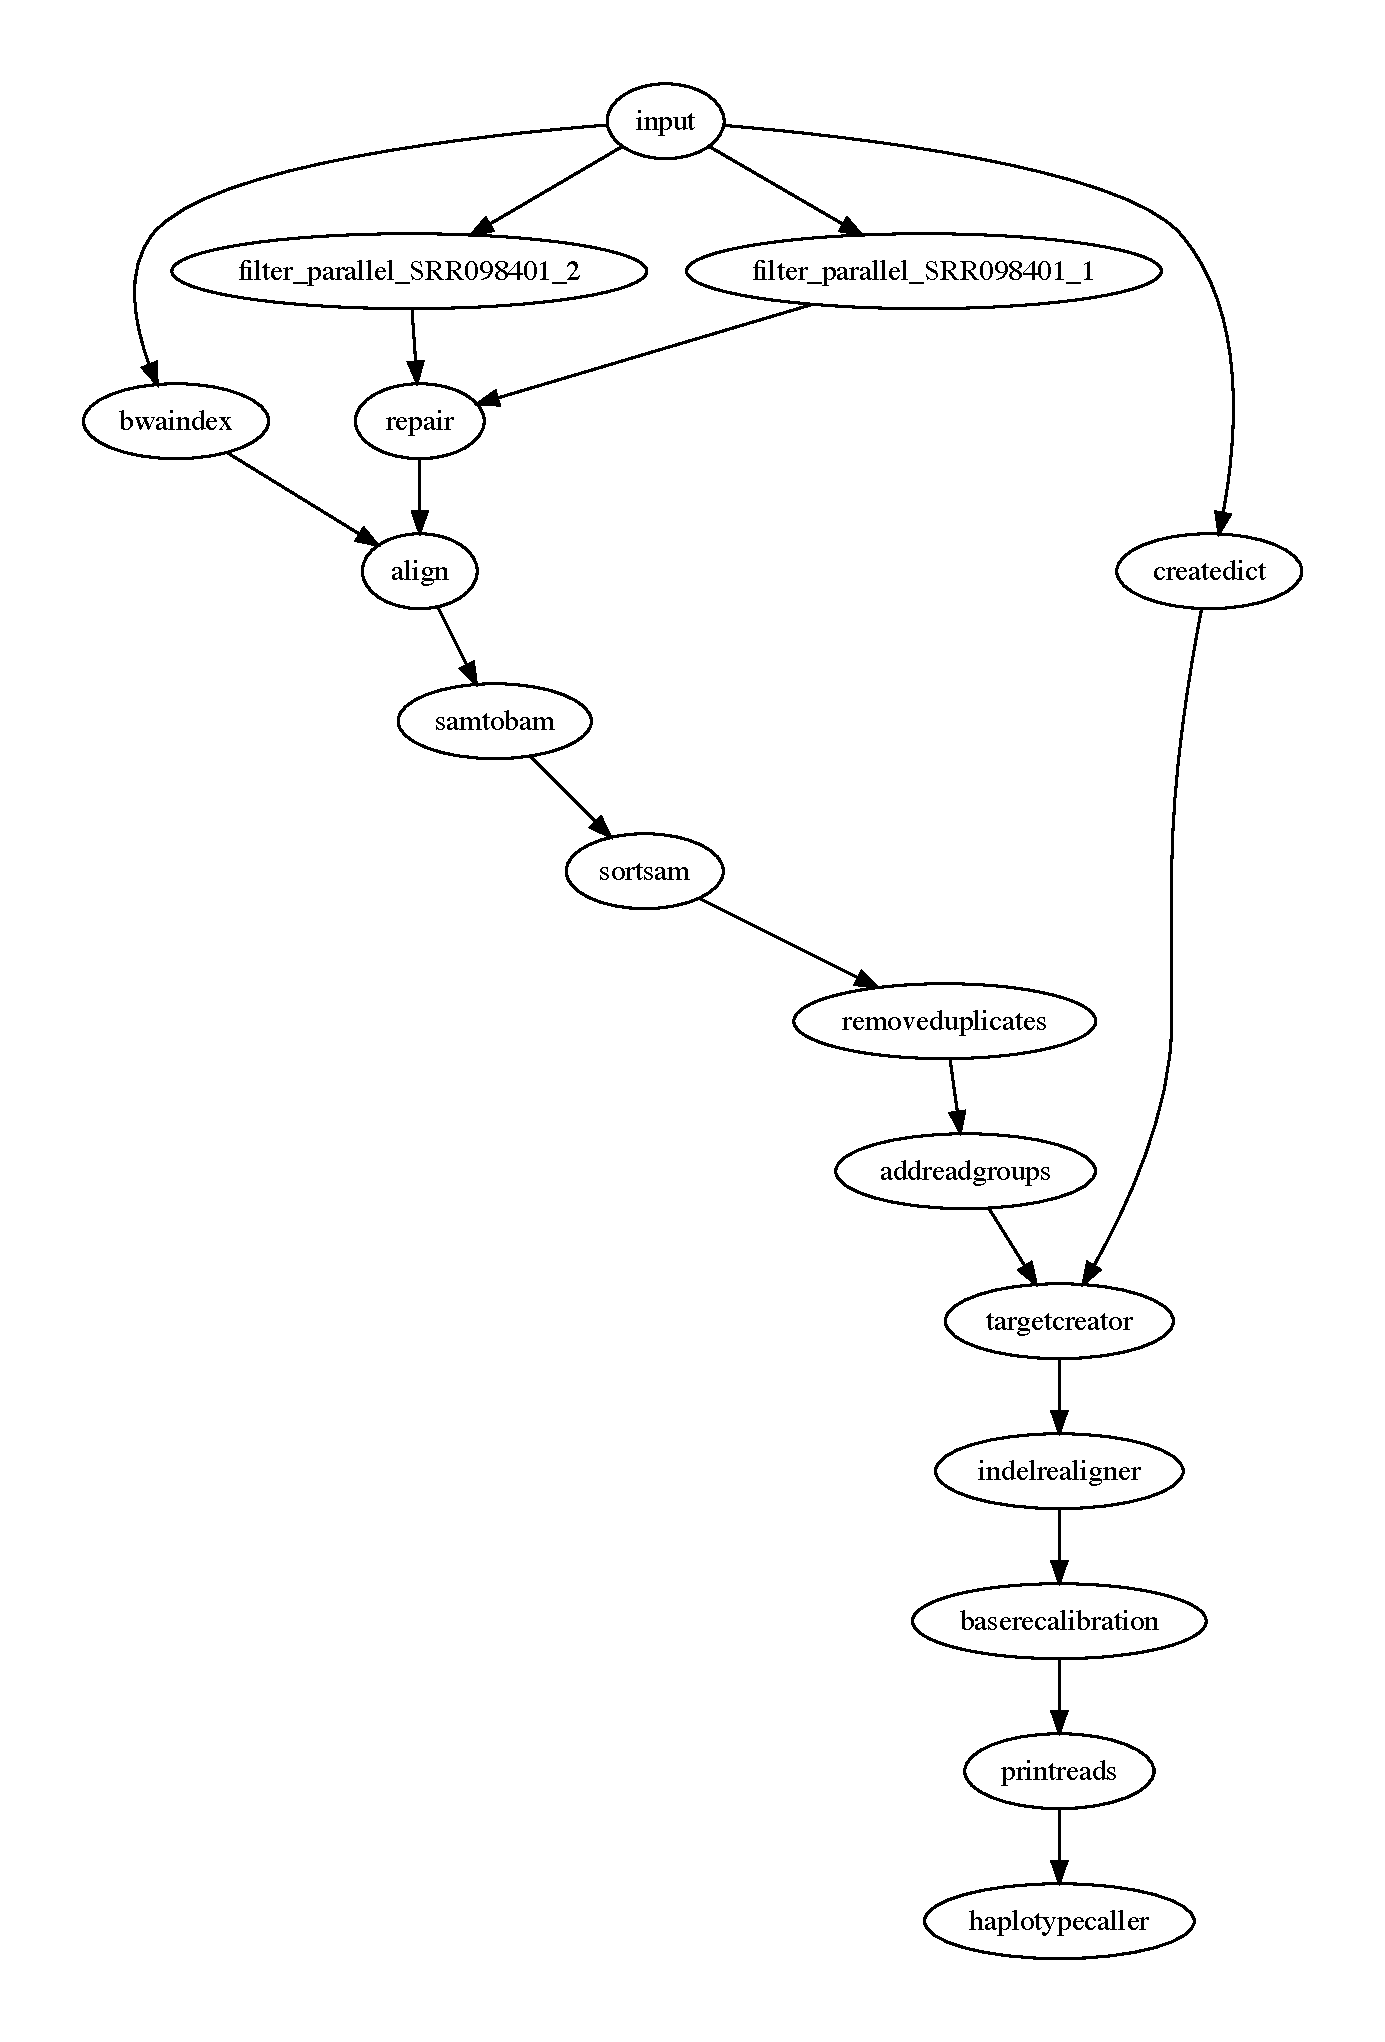
\includegraphics[width=7cm]{figures/graph.pdf}
%     \caption{WIP: Graphical representation of the example variant calling
%     pipeline.}
%     \label{benchpipefigure}
% \end{figure} 

We first run the variant calling pipeline without any additional provenance
tracking or storing of output or intermediate datasets. This is to get a
baseline performance measurement for how long we expect the pipeline to run. We
then run a second experiment to measure the overhead of versioning output and
intermediate data. Then we introduce a parameter change in one of the pipeline
steps which results in new intermediate and output datasets. Specifically we
change the \texttt{--maxReadsForRealignment} parameter in the indel realigner step
back to its default (See the online pipeline description for more
details). This forces walrus to recompute the indel realigner step
and any subsequent steps. We show the runtime and storage overhead of
introducing this pipeline change. To illustrate how walrus can restore old
pipeline configurations and results, we restore the pipeline to the initial
configuration and results. We show the computational overhead and storage usage
of restoring a previous pipeline configuration. 

Table \ref{resultstable} shows the runtime and storage use of the different
experiments. In the second experiment we can see the added overhead of adding
version control to the dataset. In total, an hour is added to the runtime and
the data size is doubled. The doubling comes from git-lfs hard copying the data
into a subdirectory of the \texttt{.git} folder in the repository. In the third
experiment we can see that only the downstream analyses from configuring the
indel realignment parameter is executed. It generates 30GB of additional data,
but the execution time is limited to the applicable stages. Restoring the
pipeline to a previous configuration is almost instantaneous since the data is
already available and git only has to modify the pointers to the correct files
in the \texttt{.git} subdirectory. 

\begin{table}[ht!]
    \centering
    \caption{Runtime and storage use of a variant-calling pipeline developed with walrus.} 
    \begin{tabular}{ | l | p{5cm} | l | l |}
    \hline
    Experiment & Task & Runtime & Storage Use \\ \hline
    1 & Run pipeline with default configuration & 21 hours 50 minutes & 235 GB \\ \hline
    2 & Run the default pipeline with version control of data & 23 hours 9 minutes & 470 GB \\ \hline
    3 & Re-run the pipeline with modified indel realignment parameter & 13 hours & 500 GB \\ \hline
    4 & Restoring pipeline back to the default configuration & < 1 second & 500GB \\ \hline
    \end{tabular}
    \label{resultstable}
\end{table}


\section{Related Work} 
There are a wealth of pipeline specification formats and workflow managers
available. Some are targeted at users with programming experience while others
provide simple \glspl{gui}.  Here we describe the most popular systems for
building data analysis pipelines. While most provide viable options for genomic
analyses, we have found most to complex to install and maintain in clinical
settings. We discuss tools that use the common \gls{cwl} pipeline specification
and systems that provide versioning of data. 

\gls{cwl} is a specification for describing analysis workflows and
tools.\cite{commonwl} A pipeline is written as a \gls{json} or \gls{yaml} file,
or a mix of the two, and describes each step in detail, e.g. what tool to run,
its input parameters, input data and output data. The pipeline descriptions are
text files that can be version controlled and shared between projects. There are
multiple implementations of \gls{cwl} workflow platforms, e.g. the reference
implementation
cwl\_runner,\footnote{\url{github.com/common-workflow-language/cwltool}}
Arvados,\cite{arvados} Rabix,\cite{rabix} Toil,\cite{toil} Galaxy,\cite{galaxy}
and AWE.\cite{awe} It is no requirement to run tools within containers, but
implementations can support it. There are few of these tools that support
versioning of the data. 
Galaxy is an
open web-based platform for reproducible analysis of large high-throughput
datasets.\cite{goecks2010galaxy} It is possible to run Galaxy on local compute
clusters, in the cloud, or using the online Galaxy site\footnote{Available at
\url{usegalaxy.org}.} In Galaxy users set up an analysis pipeline using a
web-based graphical interface, and it is also possible to export or import an
existing workflow to an \gls{xml} file.\footnote{An alpha version of Galaxy with
\gls{cwl} support is available at
\url{github.com/common-workflow-language/galaxy}.}  We chose not to use Galaxy
because of missing command-line and scripting support, along with little support
for running workflows with different configurations.\cite{spjuth2015experiences}
Rabix provides checksums of output data to verify it
against the actual output from the pipeline. This is similar to the checksums
found in the git-lfs pointer files, but they do not store the original files for
later. Arvados stores the data in a distributed storage system, Keep, that
provides both storage and versioning of data. We chose not to use \gls{cwl} and
its implementations because of its relaxed restrictions on having to use
containers, its verbose pipeline descriptions, and the complex compute
architecture required for some of the runners. We are however experimenting
with an extension to walrus that translates pipeline descriptions written in
walrus to \gls{cwl} pipeline descriptions. 

Pachyderm is a system for running  big data analysis pipelines. It provides
complete version control for data and leverages the container ecosystem to
provide reproducible data processing.\footnote{\url{pachyderm.io}} Pachyderm
consists of a file system (\gls{pfs}) and a processing system (\gls{pps}).
\gls{pfs} is a file system with git-like semantics for storing data used
in data analysis pipelines. Pachyderm ensures complete analysis reproducibility
by providing version control for datasets in addition to the containerized
execution environments. Both \gls{pfs} and \gls{pps} is implemented on top
of Kubernetes.\footnote{\url{kubernetes.io}} We believe that the approach in
Pachyderm with version controlling datasets and containerizing each pipeline
step is the correct approach to truly reproducible data analysis pipelines. 
The reason we did not use Kubernetes and Pachyderm was that it was not available
on the required in-house compute infrastructure.  

As discussed in \cite{NIK}, recent projects propose to use containers for life
science research. The BioContainers\cite{biocontainers} and
Bioboxes\cite{belmann2015bioboxes} projects addresses the challenge of
installing bioinformatics data analysis tools by maintaining a repository of
docker containers for commonly used data analysis tools.  
Docker containers are shown to have better than, or equal performance as
VMs.\cite{di2015impact} Both forms of virtualization techniques introduce
overhead in I/O-intensive workloads, especially in VMs, but introduce negligible
CPU and memory overhead.  For genomics pipelines the overhead of Docker
containers will be negligible since these tend to be compute intensive and they
typically run for several hours \cite{di2015impact}
Containers have also been proposed as a solution to improve experiment
reproducibility, by ensuring that the data analysis tools are installed with
the same responsibilities.\cite{boettiger2015introduction} 



\section{Discussion}
Precision medicine requires flexible analysis pipelines that allow researchers
to explore different tools and parameters to analyze their data. While there are
best practices to discover e.g. genomic variants, facilitating simple sharing of
pipeline descriptions, or simplifying reproducing analysis results are still
areas that need improvement. Pipelines typically need 
to be tailored to fit each project and patient, and different patients will
typically elicit different molecular patterns that require individual
investigation. While we could follow best practices to develop our pipeline we
explored different tools and parameters before we arrived at the final analysis
pipeline. 
For example, in our \gls{wes} pipeline we ran several rounds of preprocessing
(trimming reads and quality control) before we were sure that the data was ready
for analysis. Having a pipeline system that could keep track of different
intermediate datasets, along with the pipeline specification, simplifies the
task of comparing the results from pipeline tools and input parameters. While we
have developed one approach to version control genomic datasets in an analysis
pipeline, we believe that there is still room for improvement. 

While we provide one approach to version control datasets, there are still some
drawbacks. While git-lfs supports large files it
still takes a significant amount of time to add large files to a repository.
This makes the entire analysis pipeline slower, but we argue that having the
files version controlled outweigh the runtime. In addition there are as time of
writing few public hosts that allow uploads of datasets larger than a few
gigabytes. This makes it necessary to host git-lfs servers on-site and makes
sharing of full analysis repositories cumbersome. We hope that in the future
git-lfs can provide a standard way of sharing large datasets in genomics. 

We aim to investigate the performance of running analysis pipelines with walrus,
and the potential benefit of its built-in data parallelism. While
our \gls{wes} analysis pipeline successfully run steps in parallel for the
tumor and adjacent normal tissue, we have not formally investigated the benefit
of doing so. This includes benchmarking and analyzing the system requirements
for doing precision medicine analyses. 
We are also planning on exploring parallelism strategies where we
can split an input dataset into chromosomes and run some steps in parallel for
each chromosome, before merging the data again. 

\section{Conclusions} 
We have designed and implemented walrus, a tool for building reproducible data
analysis pipelines for use in precision medicine. Precision medicine requires
that analyses are run on hospital compute infrastructures and results are fully
reproducible.  By packaging analysis tools in software containers, and tracking
both intermediate and output data, walrus provides the required features to be
used in a clinical setting. 
We have used walrus to analyze a patient's metastatic lesions and adjacent
normal tissue to provide insights and recommendations for the cancer treatment. 
% LAB: Viktigere for dette paperet er å vise at walrus hjelper mht reproducibility


